%!TEX root = tesi.tex


\chapter{Three dimensional dualities}
\section{Supersymmetry and field theories in three dimensions}
Spinors in three dimensions have different properties than their four dimension counterpart.\\
The dimension of the representation in an arbitrary dimension $D$  is given by $2^{\frac{D}{2}} $
for $D$ even, while $2^{\frac{D-1}{2}} $ for $D$ odd.
Hence, in three dimension we have a two dimensional representation.
In odd dimensions representations are irreducible and Weyl spinors do not exist: the chirality operator ($\gamma_{D+1}$ or $\gamma^*$ ) is proportional to the identity.
\\
%This is related to the fact that representations in odd dimensions are constructed by taking the representation in one dimension less, which is even, and adding the chirality operator as the $D$-th matrix in the Clifford algebra.\\
Gamma matrices can be chosen real and the Majorana condition can be imposed, lowering the degress of freedom of the representation from four to two.\\
Since $3d \; \mN=2$ theories have four supercharges, we can use the $4d \; \mN=1$ superspace formalism. 
\\
The supersymmetry algebra and its representations can be found by dimensional reduction from four dimensions. 
The reduced algebra reads
\begin{equation}
 \{ Q_{\alpha},Q_{\beta} \} =  \{ \bar{Q}_{\alpha},\bar{Q}_{\beta} \}= 0 \qquad \{ Q_{\alpha} , \bar{Q}_{\beta}   \} = 2 \sigma^{\mu}_{\alpha \beta} P_{\mu} + 2 i \epsilon_{\alpha \beta} Z
 \end{equation} 
The central charge $Z$ is the component of the momentum  along the reduced direction.
Because of the presence of the central charge in the algebra, now states must satisfy a BPS bound of the form $M \geq Z $, which imply that massless representations have null central charge.
\\
The automorphism of this algebra is $U(1)_R \simeq SO(2)_R$, as in four dimensions.
\\
Superspace formalism is similar to what we introduced previously, with proper changes due to the different spinor representation in three dimension such as gamma matrices.
\\
Chiral superfields contain \emph{on-shell} one complex scalar and a complex spinor as in four dimensions.\\
Vector superfield contains an additional real scalar field with respect to the four dimensional superfield.
The scalar $\sigma $ comes from the component of the vector field $A_{\mu}$ along the reduced direction.









\subsubsection{Coulomb branch and dualized photon	}
In three dimensions a free photon can be dualized to a scalar $\gamma$ since it has only one polarization.
Instead of defining a potential $A$ in order to solve the Bianchi identity for the potential $d F = d^2 A = 0$, we can define a scalar such that
\begin{equation}
  * F = \frac{g^2}{\pi} d  \gamma  \quad \rightarrow \quad d * F  = 0  
\end{equation} 
where $*$ is the Hodge operator and $g$ is the gauge coupling.\\
The Bianchi identity $d F = 0$ can be seen as a conservation law for the topological current, which is defined as
\begin{equation}
 J_{\mu}^{top} = \frac{1}{2 \pi} * F \; =  \; \frac{1}{2 \pi} d \gamma \qquad \partial^{\mu} J_{\mu} 
\end{equation}
The topological current acts as shifts of the dualized photon $\gamma \rightarrow \gamma + \alpha$.\\
The quantization of the magnetic flux implies that the dualised photon is periodic and is normalized in such a way that $\gamma \sim \gamma + 2 \pi$.

From a vector superfield $V$ we can define a linear multiplet $\Sigma$, defined as
\begin{equation}
 \Sigma = \epsilon^{\alpha \beta} D_{\alpha} D_{\beta} V
\end{equation}
It satisfies $D^2 \Sigma = 0$ and is gauge invariant under a transformation $V \rightarrow V + i (\Phi - \Phi^{\dagger})$.
The lowest component of $\Sigma$ is the scalar in the vector multiplet and it contains also a term $ \bar{\theta} \sigma_{\rho} \theta \, \epsilon^{\mu \nu \rho} F_{\nu \rho}$, whose bosonic part is proportional to the topological current.
The super Yang-Mills action can be written also as
\begin{equation}
S \sim \int d^4 \theta \; \Sigma^2
\end{equation}
The  vacuum expectation values of scalar fields in the vector multiplet parametrize a subset of the moduli space of the theory which is called the \emph{Coulomb branch}.
Using the dualized photon we can turn the vector multiplet into a chiral multiplet, whose lowest component is a good parametrization of the Coulomb branch 
\begin{equation}
 Y = \exp{ \left( \frac{2 \pi \sigma}{g^2} + i \gamma \right)}
\end{equation}
because of its periodicty, it's natural to assign $\gamma$ to a phase factor.\\
The dualization of the photon was possible because there wasn't matter in the theory.
However, matter fields couple with $\sigma$ with mass terms. As a result, in a generic point of the Coulomb branch, all charged matter fields are massive and can be integrated out and in a low-energy description we can still dualize the gauge field.\\
We can generalize the dualization to non-Abelian gauge theories with a similar reasoning.
In a generic point of the Coulomb branch, the VEV of $\sigma$ breaks the gauge group to its maximal torus $U(1)^{r_G}$, where $r_G$ is the rank of the gauge group. 
We now have $r_G$ massless vector multiplets that can be dualized into chiral multiplets $Y_i$ with $i=1,\dotsc,r_G$.
\\
Note that since the definition of $Y$ depends on the gauge coupling, it will be modified by quantum corrections.

For $U(N)$ or $ SU(N)$ theories it's better to use the following coordinates on the Coulomb branch, since they are related to the simple roots of the algebra
\begin{equation}
 Y_k \sim \exp \left( \frac{\sigma_j- \sigma_{j+1}}{\hat{g}^2} + i ( \gamma_j - \gamma_{j+1} )   \right) \qquad \hat{g}^2 =  \frac{g^2}{4 \pi}
\label{eqn:Y_def_sun_theories}
\end{equation}
with $j = 1, \dotsc , N -1$ for $SU(N)$ or with $ j = 1, \dotsc, N$ for $U(N)$.
From now on we will fix to a Weyl chamber by setting $\sigma_1 \geq \sigma_2 \geq \dots \geq \sigma_N$ with a Weyl transformation.

\subsubsection{Real masses}

In $3 D \, \mN=2$ theories there's another way of giving a mass to a chiral multiplet other than the superpotential term $W_{mass}= m \Phi^2$, which correspond to a holomorphic mass.\\
In these theories we can couple a global symmetry, which is not a R-symmetry, to a background vector multiplet.
We will give a vacuum expectation value $\hat{m} $ to the scalar in the multiplet.
As a result, every field charged under that symmetry will receive a mass $q \, \hat{m}$, where $q$ is the charge of the field under that symmetry.
If a chiral field is charged under different global symmetry, its mass  mass is a sum of the real masses for every global symmetry that we gauged.
Real masses are parity odd and belong to vector multiplets rather than chiral fields. For this reason they cannot appear in holomorphic objects such as the superpotential.\\
In addition, real masses relative to global abelian symmetries contribute to the central charge of the supersymmetry algebra $Z$through
\begin{equation}
  Z = \sum q_i m_i
 \end{equation} 
 where $q_i$ is the charge of the field and $m_i$ the real masses under a global symmetry $U(1)_i$.\\
 Moreover, the central charge $Z$ can be promoted to a background linear superfield whose lowest component is $Z$.\\
 Another symmetry that can contribute to the central charge is $U(1)_J$, whose current is given by the linear multiplet we defined previously.
 The added term is given by $\int d^4 \theta \; V_b \Sigma $ , where $V_b$ is a background vector multiplet.
 Integrating by parts and defining  $\Sigma_b = \epsilon^{\alpha \beta} D_{\alpha} D_{\beta} V_b$ we obtain $\int d^4 \theta \; \Sigma_b V  $.
 Thus, the scalar component of the background vector field is a Fayet-Iliopulos term $\xi$, which contributes to the central charge $m_J = \xi $.

 
 
\subsubsection{Monopoles}
In three dimensions there exist finite energy solutions that can be understood in terms of four dimensional monopoles.
The scalar $\sigma$ will play the role of the scalar Higgs field in the adjoint representation typically used to introduce monopoles \cite{Weinberg:2006rq}.
Different topological solutions can be found since the scalar field at infinity must approach a vaccum solution.
Such solution doesn't have to be identical in every direction and as a result we find different topological solutions depending on how we choose to map the two-sphere at infinity to the gauge group $G$.
The mapping relates $S^2_{\infty}$ to the gauge group rather than $S^3_{\infty}$ since monopoles are localized in space rather than in space-time.\\
For a generic vacuum expectation value of $\sigma$, with $\sigma_i \neq \sigma_j$, the gauge group breaks to its maximal torus $U(1)^{r_G}$.
The possible windings around $S^2_{\infty}$ are then characterised by
\begin{equation}
 \Pi_{2} \left( G / U(1)^{r_G} \right) = \Pi_1 (U(1)^{r_G}) = \mathbb{Z}^{r_G}
\end{equation}
The equality holds if $\Pi_2(G) = 0$, which is true for every semisimple gorup and if $\Pi_1(G) = 0$, which is satisfied if the group is the covering group of the Lie algebra.
As a result there are $r_G$ different topological solutions.
Each of these solutions carry a magnetic charge for each of the $U(1)^{r_G}$ unbroken gauge fields. 
For example, for $G= SU(N_c)$ we have $N_c-1$ different topological solutions.
\\
For $SU(2)$ gauge group one solution to the equation is given by the 't Hooft-Polyakov monopole, which in singular gauge reads
\begin{equation}
  \sigma = \left( v \, \coth (v r) - \frac{1}{r} \right)  \tau^3 \qquad A_{\mu} = \epsilon_{i j 3} \hat{r}^i \left( \frac{1}{r} + \frac{v}{\sinh (vr)} \right)
\end{equation}
This solution can be easily extended to $SU(N)$ gauge group by embedding the above solutios in a $SU(2)$ subgroup of the gauge group.
Since the gauge group is broken in the vacuum, we cannot use $SU(N)$ gauge transformation to generate other solutions.
As a results, each embedding of $SU(2)$ will result in a monopole charged under different $U(1)$ factors of the Cartan. 
Note that there are $N-1$ special embeddings of $SU(2)$ into $SU(N)$ which result in monopoles charged only under one factor of the $U(1)$ in the Cartan subalgebra. They are given by the N-1 contiguous 2x2 blocks in the diagonal.\\
The carges of the monopoles can be written as
\begin{equation}
\vec{g}  = 2 \pi \sum_a n_a \vec{\alpha_a}
\end{equation}
where $\vec{\alpha_a}$ are the simple roots of the $su(N)$ Lie algebra. Dirac quantization condition imposes that $n_a \in \mathbb{Z}$.\\
Moreover, the mass of the monopoles is subject to the BPS bound which is given by
\begin{equation}
M_{monopole} \geq \frac{| \vec{g} \cdot \sigma| }{e^2} = \frac{2 \pi}{e^2} \sum_i n_i \sigma_i
\end{equation}
where $\sigma_i$ are the vaccum expectation values of $\sigma$.
Monopoles that satisfy the above condition are called BPS monopoles 
 
 
 
 
 
 \subsection{Moduli spaces of gauge theories}

\subsubsection{Moduli space of $U(1)$ gauge theory with $N_f$ massless flavours }
For large values of $\sigma$ the Coulomb branch of the theory can be parametrized by the chiral superfield we defined before $X = e^{\frac{\Phi}{g^2}} $ which correspond to a cylinder.
However, the metric for $\gamma$ receives quantum correction and thus the topology of moduli space is changed perturbatively.
The Higgs branch intersects the Coulomb branch for $\sigma=0$ and since it is invariant under $U(1)_J$, the radius of the circle must shrink to zero where they meet, since the topological symmetry acts as shifts on the circle $\gamma$.
\\
Therefore, near the origin the moduli space looks like the intersection of three cones: the Higgs branch and two cones corresponding to two distinct parts of the Coulomb branch.
Half of the Coulomb branch is parametrized semi-classically by the field $V_+ \sim e^{\frac{\Phi}{g^2}}$, while the other half by $V_- \sim e^{ -\frac{\Phi}{g^2} }$. 
Two different chiral fields are needed since near the origin the moduli space shrinks to a point and $V_+ \rightarrow 0$. 
The Higgs branch is not modified by quantum corrections and the mesons can still be used to parametrize it.\\
The charges of the fields under the symmetries are given by
 \begin{equation}
 \begin{array}{ c | c c c c c }
  & U(1)_R &  U(1)_J & U(1)_A & SU(N_f)_R & SU(N_f)_R \\
 \hline
 Q & 0 & 0  & 1 & N_f & 1  \\  
 \tilde{Q} & 0 & 0  & 1 & 1 & \overline{N_f}  \\  
   M & 0 &  0 & 2 & N_f & \overline{N_f}\\  
   V_{\pm} & N_f & \pm 1  & -N_f & 1  &  1\\
 \end{array}
\end{equation}
The symmetries force the superpotential to have the form
\begin{equation}
W = - N_f \left(  V_+ V_- \Det{ M} \right)^{\frac{1}{N_f}}
\end{equation}
The superpotential is singular at the origin of the moduli space, indicating that there are massless degrees of freedom that need to be taken into account.\\
We can give real masses $\bar{m}_i$ ($-\bar{m}_i$) to the quarks $Q_i$ ($\tilde{Q}_i$).
The Higgs branch is parametrised by the diagonal elements of $M^i_{\tilde{i}}$ which intersects the Coulomb branch at $\sigma = \bar{m}_i$.
At every intersection, we have $U(1)$ theory with one flavour.
The coulomb branch is parametrised, at every intersection, by $V_{i,\pm} = e^{\pm \frac{\Phi - \bar{m}_i}{g^2}} $ with a superpotential given by
\begin{equation}
W = - \sum_{i = 1}^{N_f} M^i_i V_{i,+} V_{i,-} + \sum_{i=1}^{N_f - 1} \lambda_i \left(    V_{i,+} V_{i+1,-} - 1\right)
\end{equation}
where $\lambda_i$ are Lagrange multipliers in order the enforce the semiclassical identification  $ V_{i,+} V_{i+1,-} = 1 $.

\begin{figure}[h!]
\centering
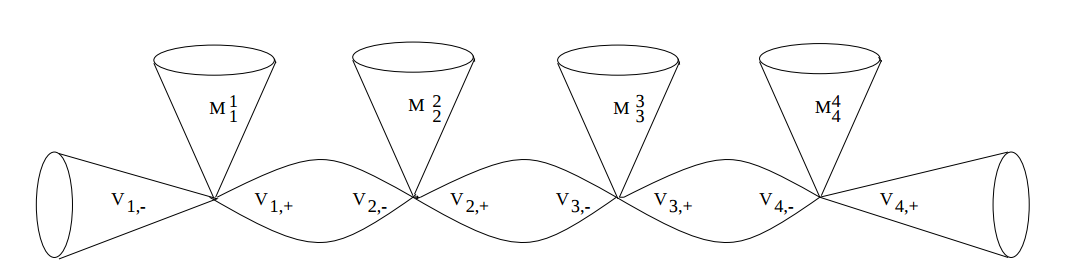
\includegraphics[scale=0.5]{u1_moduli_space_flavours.png}
\caption{Moduli space of vacua for SQED with four flavours}
\end{figure}

\begin{comment}
\subsubsection{Moduli space of $SU(2)$ gauge theories with flavours}

We will consider a $SU(2) $ gauge theories with an even number of quarks, in order to avoid the addition of Chern Simons terms.
The charges are given by
\begin{equation}
 \begin{array}{ c | c c c  c }
  & U(1)_R  & U(1)_A & SU(2 N_f)\\
 \hline
 Q & 0  & 1 & 2 N_f \\  
   M & 0 & 2 & N_f (2 N_f-1)  & \\  
   X_{\pm} & 2 N_f  -2 &  - 2 N_f & 1 \\
 \end{array}
\end{equation}
and $Y$ is defined in \eqref{eqn:Y_def_sun_theories} and parametrizes the Coulom branch.
Mesons parametrises the Higgs branch and are subject to the condition $\mathrm{rank}(M) \leq 2 $.

A theory without quarks has a superpotential, generated by instantons, that lifts completely the Coulomb branch of the theory
\begin{equation}
W = \frac{1}{Y}
\end{equation}

With $N_f = 1$ the quantum moduli space consists in a smooth merging between the Higgs and the Coulomb branch of the theory since the fields are subject to the constraint
\begin{equation}
 M \, Y = 1
\end{equation}

For $N_f \geq 2 $, there is a unique superpotential consistent with the symmetries of the theory
\begin{equation}
 W = - (N_f -1 )( Y \, \mathrm{Pf} M)^{\frac{1}{N_f -1}}
\end{equation}
For $N_f = 2$ the Higgs and Coulomb branch are distinct and they touch at $M=0 \, , \, Y=0$ instead of the point with $\sigma = 0$.
The superpotential is relevant and drives the theory to a interacting fixed point.

\end{comment}

\subsubsection{Moduli spaces for $SU(N_c)$ theories with $N_f$ flavours}
We will consider a $SU(N_c)$ gauge theory with equal number of $Q$ and $\tilde{Q}$ in order to avoid Chern-Simons term. 
The simmetries of the theory are given by the following table

 \begin{equation}
\begin{array}{ c | c c c c c}
  & U(1)_R & U(1)_B & U(1)_A & SU(N_f)_L & SU(N_f)_R \\
 \hline
 Q & 0 &1 & 1 & N_f & 1 \\  
 \tilde{Q}& 0 &-1 & 1 &1 & \overline{N_f}  \\  
   M & 0 & 0 & 2 & N_f & \overline{N_f}\\  
   Y_{j \neq K} & -2 & 0  & 0 &  1 & 1 \\
   Y_{K} & 2 (N_f -1 ) & 0 & - 2 N_f & 1 & 1 \\
   Y & 2 ( N_f -N_c +1) & 0 & - 2 N_f & 1 & 1 \\
\end{array}
\end{equation}
where $Y_j$ are defined as in \eqref{eqn:Y_def_sun_theories} and $Y$ is defined as $Y = \prod_{j=1}^{N_c -1} Y_j \sim e^{ \frac{ \Phi_1 - \Phi_{N_c}  }{g^2}}$.
The adjoint scalar VEV is ordered in such a way that $ \sigma_1 \geq \sigma_2 \geq \dotsc \geq \sigma_{N_c}$. The value of $j$ for which $\sigma$ changes sign is called $K$ and the associated instanton is $Y_K$.
For $N_f > 1$ the theory has a Higgs branch, which break the gauge group in a generic point to $SU(N_f -N_c)$ for $N_f <N_c -1 $ and completely for $N_f \geq N_c - 1$. 
The Higgs branch is parametrised as in four dimensions by mesons and for $N_f \geq N_c$ also by baryons.

For theory withouth quarks, instantons generate the Affleck-Harvey-Witten \cite{Affleck:1982as} superpotential
\begin{equation}
W = \sum_{j=1}^{N_c - 1} \frac{1}{Y_j}
\end{equation}
which prohibits the theory to have stable supersymmetric vacuas.

The theory with massless quarks features a superpotential generated by $N_c - 2$ instantons 
\begin{equation}
W_{inst} = \sum_{j \neq K} \frac{1}{Y_j}
\end{equation}
which doesn't completely lift the Coulomb branch.
In fact, the following subspace is classically unlifted
\begin{equation}
 \sigma_1 > \sigma_2 = \dots = 0 > \sigma_{N_c} = - \sigma_1
\end{equation}
The last equality holds since for $SU(N_c)$ we have $\sum_i \sigma_i = 0$.
The quantum corrected moduli space is different from the classical one and for $N_f < N_c -1 $ the effective superpotential is given by
\begin{equation}
 W_{eff} = (N_c - N_f - 1) ( Y \Det{M} ) ^{\frac{1}{N_f - N_c +1}}
\end{equation}
which admits no stable vacuum.\\
For $N_f = N_c - 1 $ we obtain a constraint on the moduli space given by 
\begin{equation}
Y \Det M = 1
\end{equation}
which results in a merging between the Higgs and the Coulomb branch.

For $N_f \geq N_c $, the low-energy description contains baryons.
In the $N_f = N_c$ case the superpotential is 
\begin{equation}
W = - Y ( \Det{M} - B \tilde{B})
\label{eqn:3d_sun_nf__n_c_superpot}
\end{equation}
which forces the theory to flow to a non-trivial fixed point in the infrared.

The above analysis can be extended to theories with $U(N_c)$ gauge group with $N_f \leq N_c$.
We will discuss the theory with $N_f = N_c$ since the results with lower number of flavours can be obtained by integrating out quarks.\\
The theory with $U(N_c)$ is obtained by gauging the global $U(1)_B$ factor.\\
Since we have $N_f=N_c$ the superpotential \eqref{eqn:3d_sun_nf__n_c_superpot} from the $SU(N_c)$ part of the group is presenet  and for the $U(1)$ factor we have one flavour given by $X = B \tilde{B}$ 
and chiral fields $V_+ \, , \,V_-$ which results in a superpotential given by
 $$ W = - X V_+ V_-$$.
The fields $V_+ \, , \, V_-$ are defined as 
\begin{equation}
V_+ \sim \exp{ \left(  \frac{\Phi_1}{g^2} + i \gamma_1 \right) } \qquad \quad V_- \sim \exp{ \left( \frac{\Phi_{N_c}}{g^2} + i \gamma_{N_c} \right) }
\end{equation}
since the null trace condition does not hold anymore.\\
The complete superpotential now reads
\begin{equation}
 W = - Y ( \Det{M}  - X) - X V_+ V_- 
 \end{equation} 
Integrating out the massive field $Y$  we obtain a superpotential

\begin{equation}
W = -  V_+ V_-  \Det{M}
\end{equation}



\section{Aharony duality}
One of the first three dimensional dualities was found by Aharony in \cite{Aharony:1997gp} for theories with $U(N_c) $ as gauge group and with non chiral matter in the fundamental representation.
The charges of the fields are given by the following table
\begin{equation}
\begin{array}{ c | c c c c c}
  & U(1)_R & U(1)_A & U(1)_J  & SU(N_f)_L & SU(N_f)_R \\
 \hline
 Q & 0 & 1 & 0 & N_f & 1 \\  
 \tilde{Q}& 0  & 1 & 0  & 1 & \overline{N_f}  \\  
   M & 0  & 2 & 0& N_f  & \overline{N_f}\\  
  V_{\pm} & N_f - N_c + 1 & - N_f  & \pm 1 &  1 & 1 \\
\end{array}
\end{equation}
where $V_{\pm} $ are defined as in the previous section and parametrize the unlifted Coulomb branch.
The moduli space of this theory was described in the previous section.









\section{Kutasov-Schwimmer duality}
